\documentclass{article}
\usepackage[margin=0.9in]{geometry}
\usepackage[utf8]{inputenc}
\usepackage[T1]{fontenc}
\usepackage{textcomp}
\usepackage{gensymb}
\usepackage{enumitem}
\usepackage{physics}
\usepackage{graphicx}
\usepackage{siunitx}
\usepackage{amsmath}
\usepackage{amssymb}
\usepackage[dvipsnames, table]{xcolor}
\usepackage[sort&compress, round]{natbib}
\usepackage{bm}
\usepackage{url}
\usepackage{xr-hyper}
\usepackage{hyperref}
\usepackage{parskip}
\usepackage{lineno}
\usepackage{float}
\usepackage{appendix}
\usepackage[font=small,skip=5pt]{caption}

%\linenumbers

%%% WORD COUNTING
\usepackage{verbatim}

\newcommand{\detailtexcount}[1]{%
  \immediate\write18{texcount -merge -sum -q #1.tex output.bbl > #1.wcdetail }%
  \verbatiminput{#1.wcdetail}%
}

\newcommand{\quickwordcount}[1]{%
  \immediate\write18{texcount -1 -sum -merge -q #1.tex output.bbl > #1-words.sum }%
  \input{#1-words.sum} words%
}

\newcommand{\quickcharcount}[1]{%
  \immediate\write18{texcount -1 -sum -merge -char -q #1.tex output.bbl > #1-chars.sum }%
  \input{#1-chars.sum} characters (not including spaces)%
}
%%%%%%

\setlength\parindent{0pt}
\renewcommand{\baselinestretch}{1.5}

\newcommand{\TODO}[1]{\todo[inline,backgroundcolor=red!25,bordercolor=red]{#1}}
\newcommand{\alan}[2][]{\todo[color=green, #1]{\textbf{Alan}: #2}}
\newcommand{\henri}[2][]{\todo[color=orange, #1]{\textbf{Henri}: #2}}
\usepackage[obeyFinal,textsize=footnotesize]{todonotes}


\usepackage{authblk}

\title{Linear Analysis, Non-linear Simulation, and Parameterization of Submesoscale Baroclinic Instabilities in Bottom Frontal Zones}
\author[1,c]{Henri F. Drake}
\author[1]{Sonya Legg}
\affil[1]{Princeton University, Princeton, NJ, USA}
\affil[c]{\normalfont{Corresponding author: henrifdrake@gmail.com}}


\date{}             %% if you don't need date to appear
\setcounter{Maxaffil}{0}
\renewcommand\Affilfont{\itshape\small}

\begin{document}

\maketitle

\linenumbers
\begin{abstract}
    TBD
\end{abstract}
%TC:endignore

%\quickwordcount{main}
% \quickcharcount{main}
%\detailtexcount{main}

\section{Spin-Down of the Bottom Frontal Zone}

Consider the basic state illustrated in Figure \ref{fig:BML-scales} which consists of a geostrophically-balanced front along a sloping boundary (with slope angle $\theta$). We assume this Bottom Frontal Zone (BFZ) only extends a distance $H_{\text{BFZ}}$ above the boundary (or a slope-normal distance of $H_{\text{BFZ}} \cos{\theta}$), corresponding to a horizontal frontal width of $L_{\text{BFZ}} = H_{\text{BFZ}} \cot{\theta}$. For simplicity, we assume the BFZ frontal strength is uniform within the BML, i.e.~$\overline{\mathcal{B}}_{\hat{x}} = M^{2}$. The BFZ matches to a uniformly-stratified interior (i.e.~$\overline{\mathcal{B}} = N^{2}\hat{z}$) with a barotropic along-slope flow determined by matching with the frontal zone thermal wind shear ($f \hat{V}_{\hat{z}} = \mathcal{B}_{\hat{x}}$) and no-slip bottom boundary condition. It is useful to decompose the buoyancy field to separate the background stratification from the frontal zone adjustment in the BML, $B = N^{2}\hat{z} + b$. Continuity of buoyancy surfaces across the top of the BML ($\eta=H$) implies the BML stratification is reduced by $b_{\hat{z}} = -M^{2} \cot{\theta} \mathcal{H}(H-\eta)$, where $\mathcal{H}(\eta)$ is the Heaviside function. Isopycnal slopes are given by $s \equiv -B_{x}/B_{z} = \tan{\theta} (1 - \alpha)^{-1}\mathcal{H}(H-\eta)$ where $\alpha \equiv N^{2} M^{-2} \tan{\theta}$ is the slope parameter.


\begin{figure}[htb!]
\noindent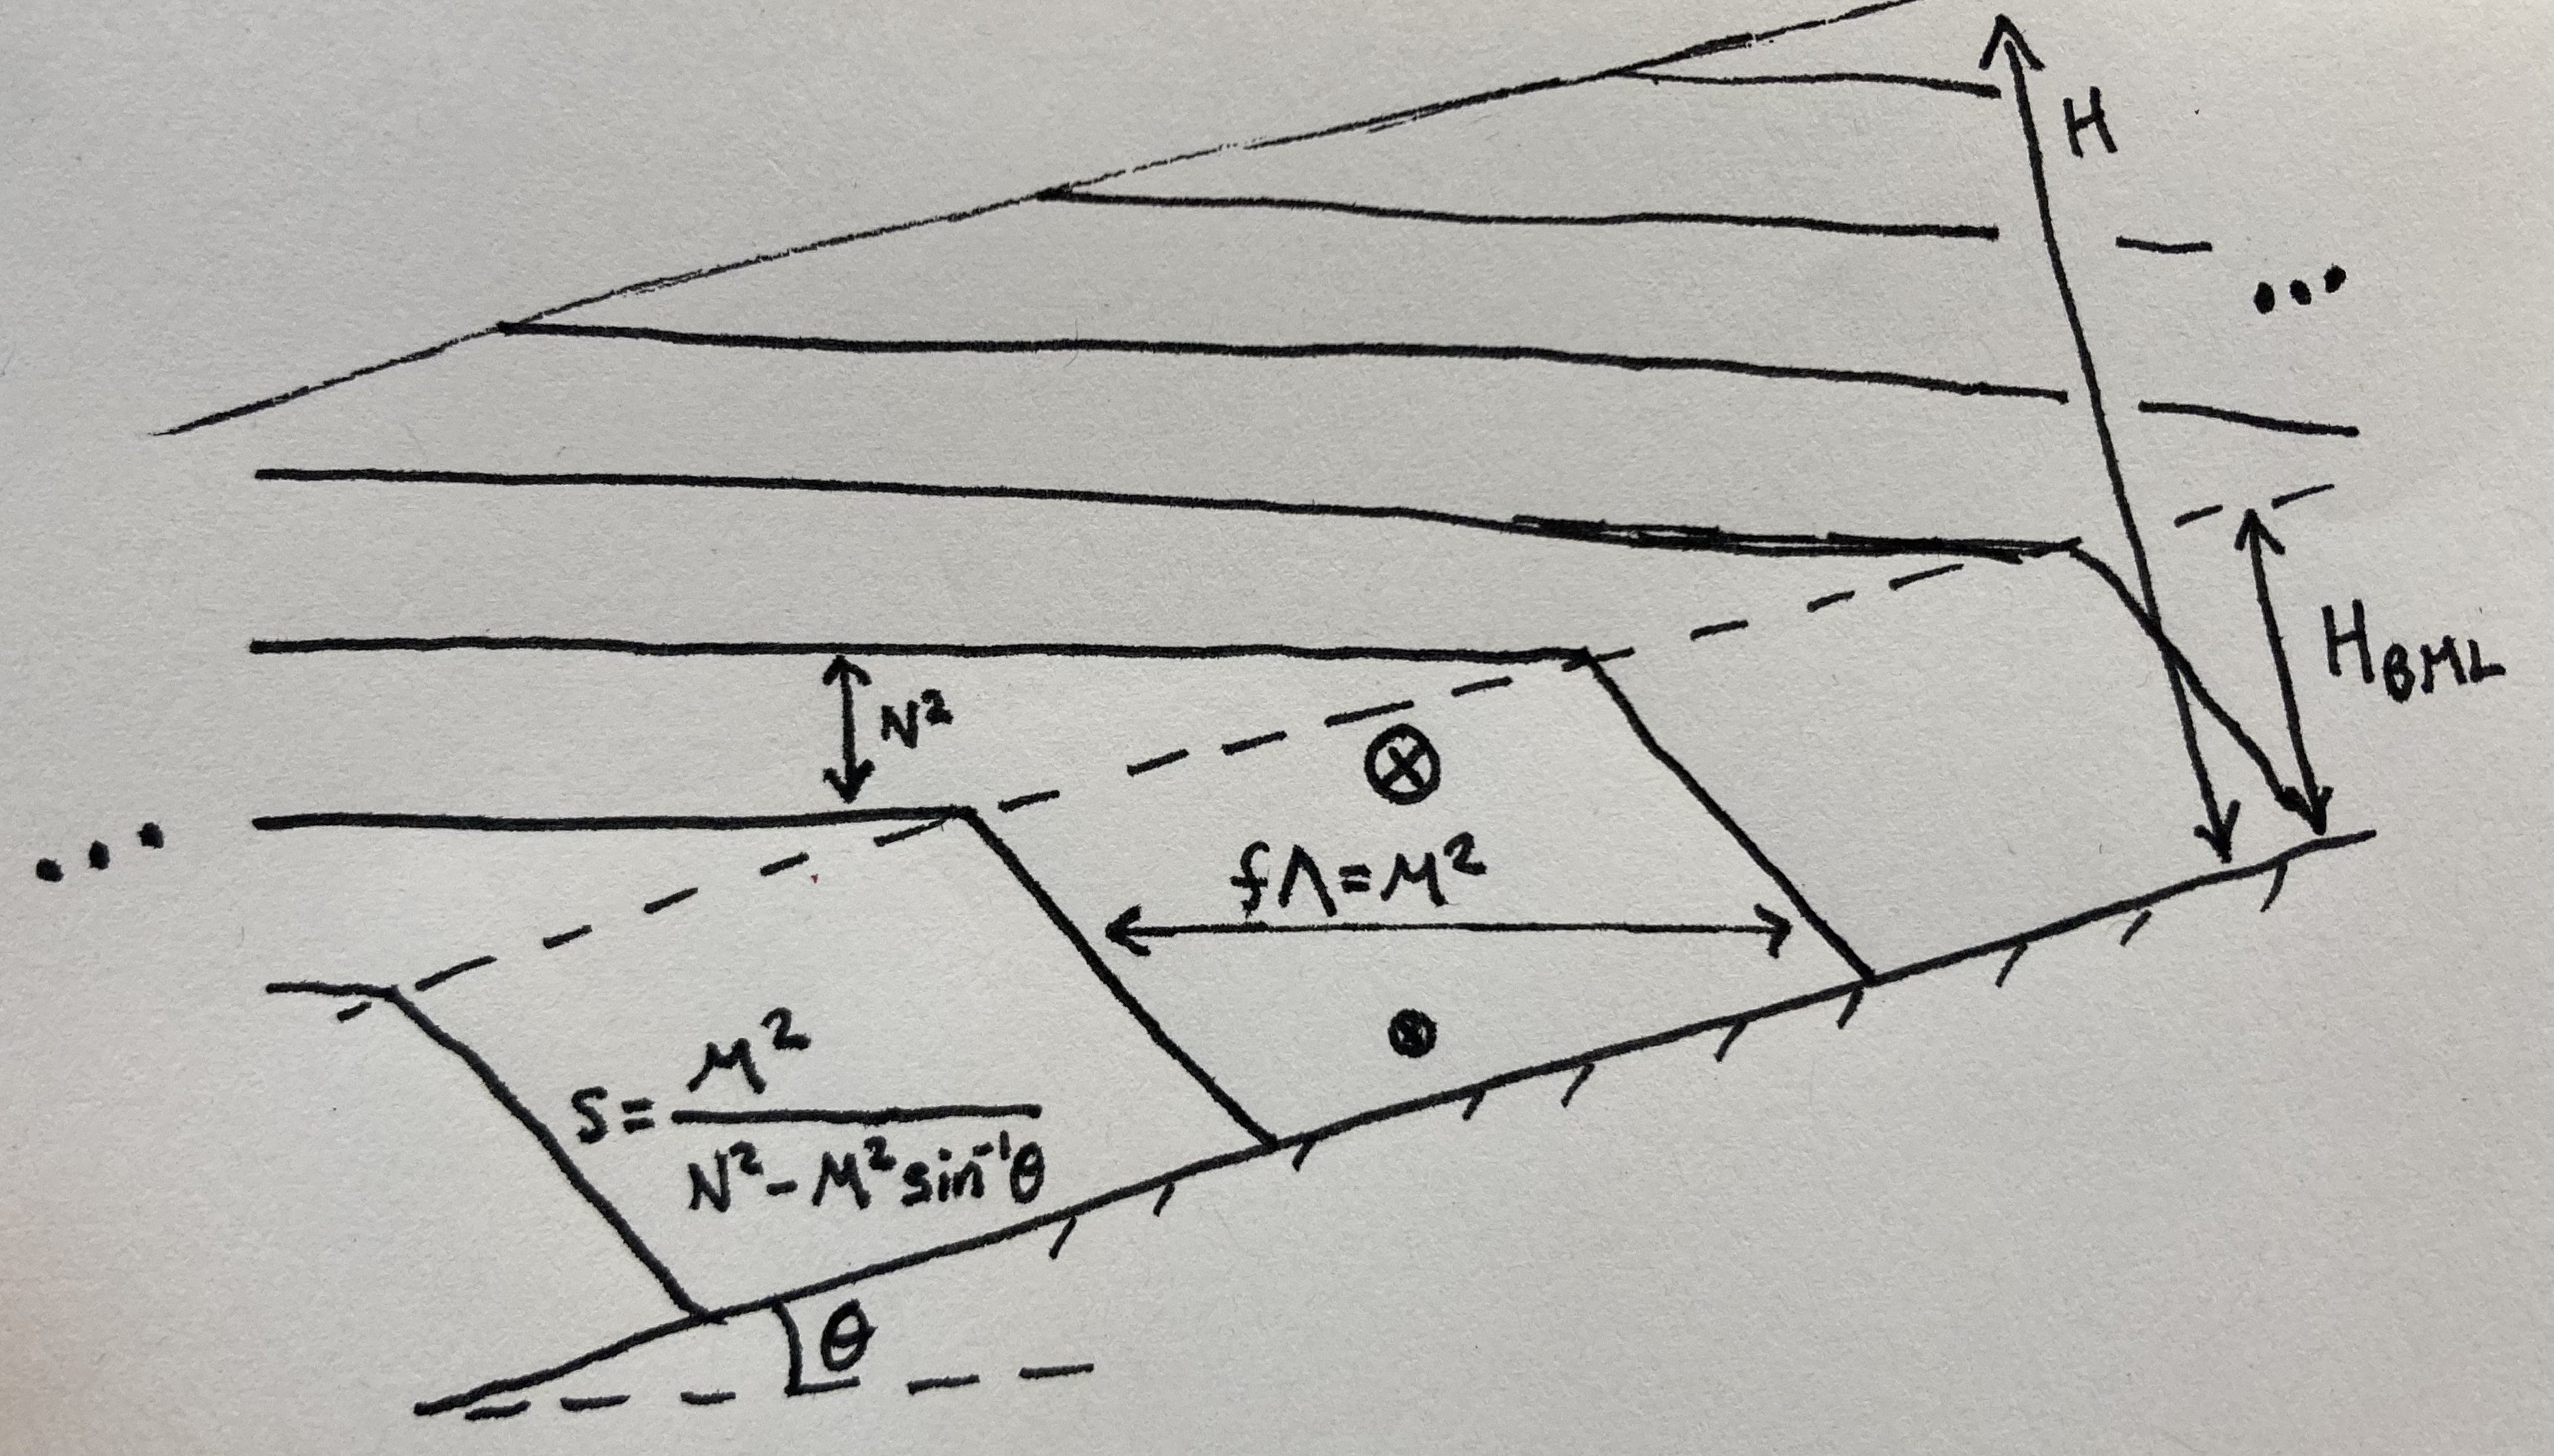
\includegraphics[width=0.75\textwidth]{overleaf/BML_scales.png}
\centering
\caption{.}
\label{fig:BML-scales}
\end{figure}

\section{Equilibrium Bottom Frontal Zones}

The equilibration of BFZs ultimately occurs on the glacial timescales of weak interior mixing, $\tau \sim \kappa_{\text{BG}}/H^{2} = \SI{1000}{years}$, and is thus challenging to achieve at the higher resolutions needed to resolve the eddy field \citep{drake_dynamics_2022}. However, because the eddies are trapped to the vigorously mixed BFZs, the interior regions of eddying solutions tend to be well-predicted by the interior solution of 1D non-eddying models. Thus, by initializing the eddying solutions with infinitesimally-perturbed steady-state 1D solutions, we can dramatically accelerate the approach to a statistical equilibrium.

\section{Linear stability analysis of BFZs}

The hydrostatic\footnote{For the reference BFZ parameters, I found that including non-hydrostatic terms in the linear stability calculations had a negligible effect on growth rates.} Boussinesq equations are given by
\begin{gather}
\hat{U}_{t} + \hat{\mathbf{U}} \cdot \nabla \hat{U} -f\hat{V} = -P_{\hat{x}} +  \nabla \cdot (\nu \nabla \hat{U}) \\
\hat{V}_{t} + \hat{\mathbf{U}} \cdot \nabla \hat{V} +f\hat{U} = -P_{\hat{y}} +  \nabla \cdot (\nu \nabla \hat{V}) \\
P_{\hat{z}} = \mathcal{B} \\
\nabla \cdot \hat{\mathbf{U}} = 0 \\
\mathcal{B}_{t} + \hat{\mathbf{U}} \cdot \nabla \mathcal{B} = \nabla \cdot \left( \kappa \nabla \mathcal{B} \right),
\end{gather}
where $\hat{\mathbf{U}}=(\hat{U},\hat{V},\hat{W})$ is the velocity vector in the usual coordinates (i.e.~such that the vertical is aligned with gravity). In the context of BFZs over sloping topography, it is more convenient to work in the slope-aligned coordinates $(x,y,z)=(\hat{x}\cos{\theta} + \hat{z}\sin{\theta}, \hat{y}, \hat{z}\cos{\theta} - \hat{x}\sin{\theta})$.

In slope-aligned coordinates, we have, for small slopes ($\tan{\theta} \ll 1$),
\begin{gather}
U_{t} + \mathbf{U} \cdot \nabla U -fV\cos{\theta} = -P_{x} + \mathcal{B}\sin{\theta} +  \nabla \cdot (\nu \nabla U) \label{eq:slope-aligned-x-momentum} \\
V_{t} + \mathbf{U} \cdot \nabla V +fU\cos{\theta} = -P_{y} + \nabla \cdot (\nu \nabla V) \\
P_{z} = \mathcal{B}\cos{\theta} \\
\nabla \cdot \mathbf{U} = 0 \\
\mathcal{B}_{t} + \mathbf{U} \cdot \nabla \mathcal{B} = \nabla \cdot \left( \kappa \nabla \mathcal{B} \right), \label{eq:slope-aligned-buoyancy}
\end{gather}

We decompose the buoyancy field as $\mathcal{B} = N^{2}\hat{z} + B$. We define the overbar operation, $\overline{\Phi}$, as a large-scale average along the sloping $(x,y)$ plane. These large-scale averages are the basic states upon which we anticipate smaller-scale instabilities might occur. We denote the smaller-scale departures from this average basic state by lower-case variables, e.g.~$\Phi = \overline{\Phi} + \phi$. We assume the perturbations are initially small, allowing us to linearizing equations \ref{eq:slope-aligned-x-momentum}-\ref{eq:slope-aligned-buoyancy} by ignoring non-linearly products of the fluctuations.

After subtracting the linearized evolution equations for the mean, we are left with the residual evolution equations for the fluctuations:
\begin{gather}
u_{t} + w \overline{U}_{z} + \overline{U}u_{x} + \overline{V}u_{y} - f v\cos{\theta} = -p_{x} + b\sin{\theta} +  \nabla \cdot (\nu \nabla u) \\
v_{t} + w \overline{V}_{z} + \overline{U} v_{x} + \overline{V} v_{y} + fu\cos{\theta} = -p_{y} + \nabla \cdot (\nu \nabla v) \\
p_{z} = b \cos{\theta} \\
\nabla \cdot \mathbf{u} = 0 \\
b_{t} + (w\cos{\theta} + u\sin{\theta})N^{2} + w \overline{B}_{z} + \overline{U} b_{x} + \overline{V} b_{y} = \nabla \cdot \left( \kappa \nabla b \right).
\end{gather}

We assume the fluctuations take the form of normal modes with some to-be-determined slope-normal structure, $\phi(x,y,z,t) = \phi(z) e^{i(kx+\ell y-\omega t)} + \text{cc}$. For a fixed wavenumber vector $(k,\ell)$, this reduces to an eigenvalue problem for the largest growth rate (i.e.~the eigenvalue $\omega$ with the largest imaginary component $\Im{\omega}$) and its corresponding eigenvectors $\phi(z)$.


\subsection{Sensitivity to friction}

%TC:ignore
%\section{Acknowledgments}

%TC:endignore

\newpage

\bibliographystyle{plainnat}
\bibliography{references}

\end{document}